


\begin{frame}{Udsætning af fasaner}

\begin{columns}[T] % T = top-aligned

\begin{column}{0.48\textwidth}
\textbf{Regler ved udsætning af fasaner:}
\begin{itemize}
    \item Kan udsættes 1. april til 31. august 
    \item Under 100ha max 100 fugle
    \item Over 100ha 1 fugl pr ha
    \item Biotopplan implementeret op til 7 fugle pr ha
    \item 5 årig biotopplan 2 år inde implementeret op til 12 fugle pr ha
    \item Afvigelser fra 1 fugle pr ha afhænger af pointsystem
    \item Alle udsætninger skal indberettes senest 1 uge efter udsætningen
\end{itemize}
\end{column}

\begin{column}{0.3\textwidth}
    % Vælg én af disse – de ser godt ud i præsentation
    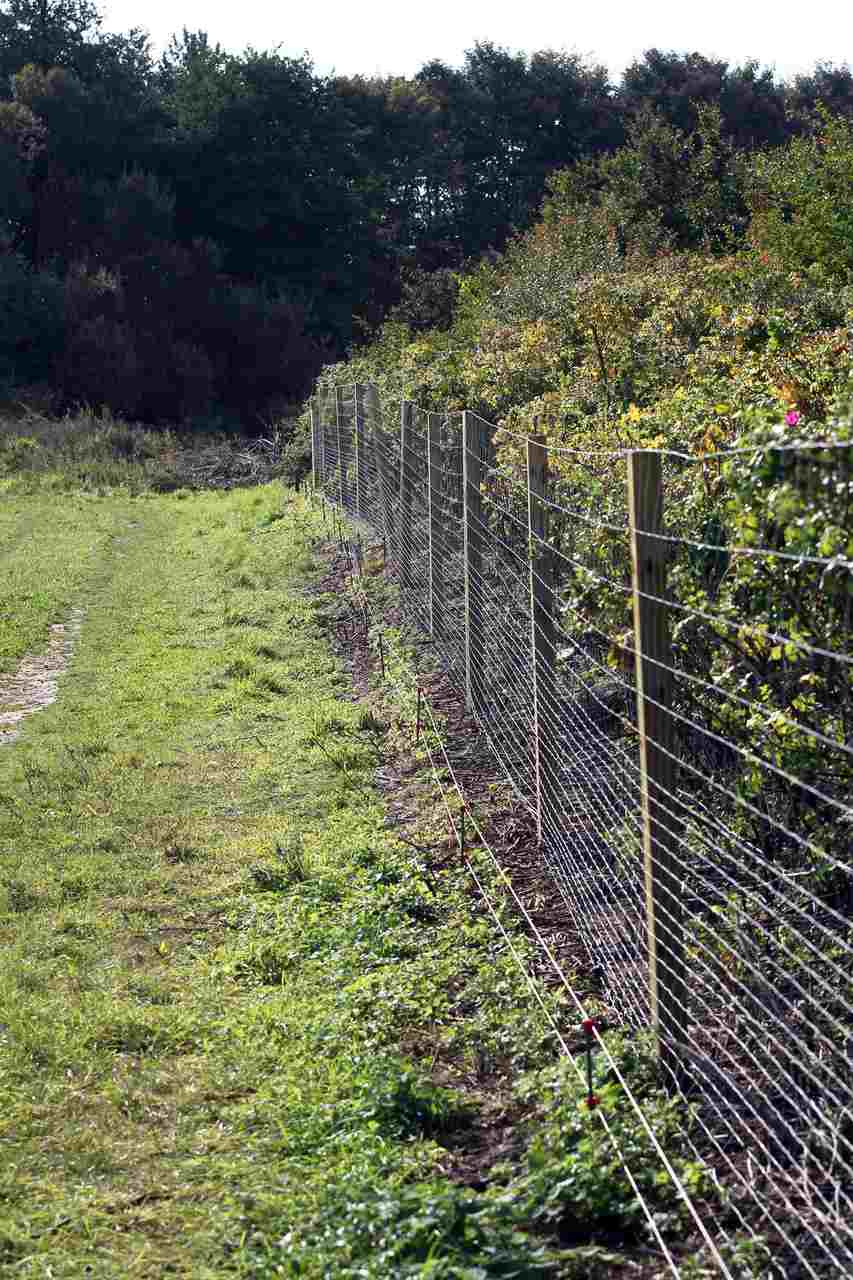
\includegraphics[width=\textwidth]{Billeder/Vildtforvaltning/udsætning/fasanvoilere.jpg}
    % Eller brug et af de gode eksempler:
    % \includegraphics[width=\textwidth]{vegetationsstriber_midtmark_ex.jpg}
\end{column}

\end{columns}

\end{frame}